\documentclass[12pt, a4papre]{article}
\usepackage[catalan]{babel}
\usepackage[unicode]{hyperref}
\usepackage[dvipsnames]{xcolor}
\usepackage{amsmath}
\usepackage{amssymb}
\usepackage{amsthm}
\usepackage{xifthen}
\usepackage{siunitx}
\usepackage{xcolor}
\usepackage{float}
\usepackage{listings}
\usepackage{setspace}
\usepackage{graphicx}
\usepackage{tikz,lipsum,lmodern}
\usepackage[most]{tcolorbox}
\usepackage{multicol}
\usepackage{fancyvrb}
\usepackage{circuitikz}
\usepackage{indentfirst}
\usepackage{verbatimbox}
\usepackage{verbatim}
\usepackage[utf8]{inputenc}
\definecolor{mygreen}{RGB}{28,172,0} % color values Red, Green, Blue
\definecolor{mylilas}{RGB}{170,55,241}
\graphicspath{ {./Images/} }

\newcommand{\norm}[1]{\lvert #1 \rvert}

\hypersetup{
    colorlinks = true,
    linkcolor = blue
}
\newtheorem*{theorem*}{Theorem}
\newtheorem*{lemma}{Prop}

\usepackage{xcolor}
\usepackage{listings}
\lstloadlanguages{Python}
\lstset{
  language=Python,
  basicstyle=\scriptsize\sffamily,
  numberstyle=\color{gray},
  stringstyle=\color[HTML]{933797},
  commentstyle=\color[HTML]{228B22}\sffamily,
  emph={[2]from,import,pass,return}, emphstyle={[2]\color[HTML]{DD52F0}},
  emph={[3]range}, emphstyle={[3]\color[HTML]{D17032}},
  emph={[4]for,in,def}, emphstyle={[4]\color{blue}},
  showstringspaces=false,
  breaklines=true,
  prebreak=\mbox{{\color{gray}\tiny$\searrow$}},
  numbers=left,
  xleftmargin=15pt
}

\author{Daniel Vilardell}
\title{Exercici Compressió d'Imatge amb Metodes de Factorització}
\date{Abril 2021}

\begin{document}
	\maketitle

	\section{Sessió 1}
		
	Executant el codi es poden trobar 9 compressions amb diferents valors de $k$ per cada una de les factoritzacions, on es pot veure clarament quines es conserven millor i pitjor. Aquí al document mostrarem les diferents imatges obtingudes amb el seu error corresponent per el valor de $k=300$.
	
	\begin{figure}[H]
		\begin{center}
		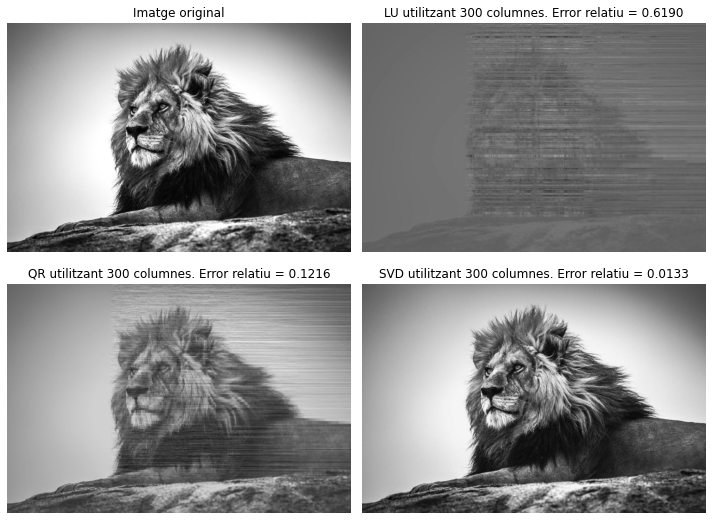
\includegraphics[width=110mm]{img_3_1.png}
		\caption{Compressió amb diferents factoritzacions}
		\end{center}
	\end{figure}
	
	\section{Sessió 2}
	
	El error relatiu de la descomposició SVD es pot trobar com 
	\[
		error = \frac{||A-ASVD||_2}{||A||_2}
	\]
	
	On $||A||_2$ es la norma matricial que es igual al valor singular mes gran de $A$. Una forma de trobarho seria trobar primer els vaps de $A^TA$ i despres fer la arrel quadrada del vap mes gran. La norma de $||A-ASVD||_2$ sera el k-essim vap mes gran on $k$ es el nombre de columnes i files que s'agafen de $A$ al fer la factorització amb $ASVD$.
	
	El cost d'emmagatzemar una imatge representada per $nxm$ pixels sera
	
	\[
		cost = 64\cdot (n\cdot k + k + m\cdot k) = 64 k\cdot (n + m + 1) 
	\]
	
	\begin{figure}[H]
		\begin{center}
		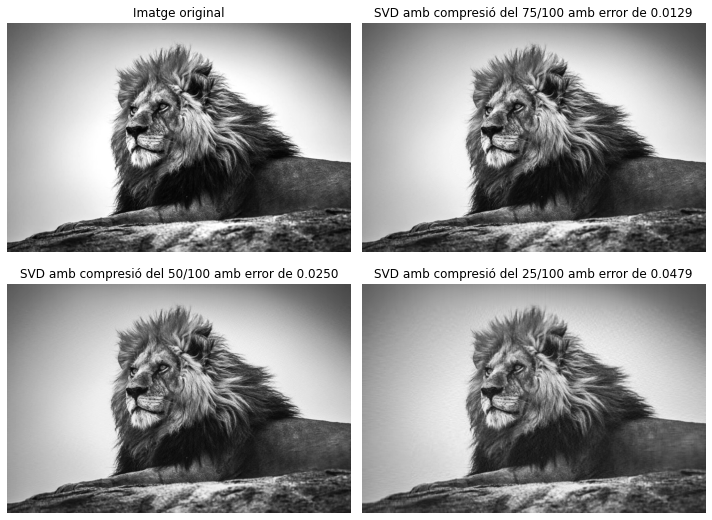
\includegraphics[width=130mm]{img_3_2.png}
		\caption{Diferents nivells de compressio amb SVD}
		\end{center}
	\end{figure}
	\newpage
	
	\section{Sessió 3}
	
	Usant la mateixa forma per a trobar les columnes i files que es necessiten per a comprimir una imatge un $p\%$ i a partir de la formula que calcula l'error donada per el enunciat obtenim les seguents 3 imatges, junt amb l'original.
	
	\begin{figure}[H]
		\begin{center}
		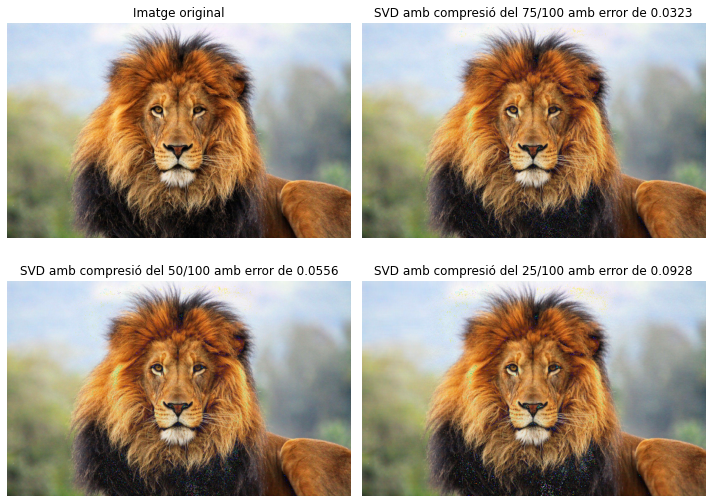
\includegraphics[width=130mm]{img_3_3.png}
		\caption{Diferents nivells de compressio amb SVD}
		\end{center}
	\end{figure}
	
	
\end{document}
